\level{1}{Pianificazione}
Di seguito saranno elencate le durate e le caratteristiche di ogni fase. I tempi sono stati pensati per permettere uno slack sufficiente per abbassare i rischi relativi alle tempistiche.
	% !TEX encoding = UTF-8 Unicode
\subsection{Fase A}
	\textbf{Periodo}: dal \insdate{25}{11}{2014} al \insdate{23}{01}{2015} \\
	Questa fase comincia con la presentazione in aula delle “Regole del progetto didattico”. Essa termina con la scadenza della consegna della \insrev{Revisione dei Requisiti}.\\Le sottofasi sono le seguenti:
	\begin{description}
		\item[Individuazione/creazione strumenti]: In questa sottofase vengono scelti gli strumenti che saranno utilizzati per la stesura dei documenti, per il tracciamento dei requisiti e alcuni script di controllo dei documenti. Se alcuni di essi non sono disponibili nella rete o non soddisfacenti, verranno creati su misura.
		\item[Norme di Progetto]: Dopo aver individuato gli strumenti si potrà procedere alla stesura del documento \insfile{Norme Di Progetto 1.0}. Questo documento sarà utilizzato indipendentemente dal capitolato che sarà preso in appalto.
		\item[Creazione documentazione]: In questa fase sappiamo esattamente con cosa e in che modo dobbiamo scrivere un documento e possiamo iniziare la stesura dei documenti.
			\begin{itemize}
				\item \textbf{Studio di Fattibilità}: Vengono valutati pro e contro di tutti i capitolati proposti e viene redatto il documento \insfile{Studio Di Fattibilità 1.0}. Viene quindi scelto il capitolato da sviluppare.
				\item \textbf{Analisi dei Requisiti}: Viene steso il documento \insfile{Analisi Dei Requisiti 1.0}. Prima e durante la stesura di questo documento verranno fatti degli incontri con il proponente per consolidare i requisiti stesi o per chiarire le idee sui requisiti da stendere.
				\item \textbf{Piano di Progetto}: Si stende il documento \insfile{Piano Di Progetto 1.0} per regolare le attività che il team dovrà svolgere.
				\item \textbf{Piano di Qualifica}: Si redige il documento \insfile{Piano Di Qualifica 1.0}.
				\item \textbf{Glossario}: viene incrementato il file  \insfile{Glossario.xml} e steso in modo automatico il documento \insfile{Glossario 1.0}.
			\end{itemize}
	\end{description}
	\subsubsection{Diagramma di Gantt delle attività}
		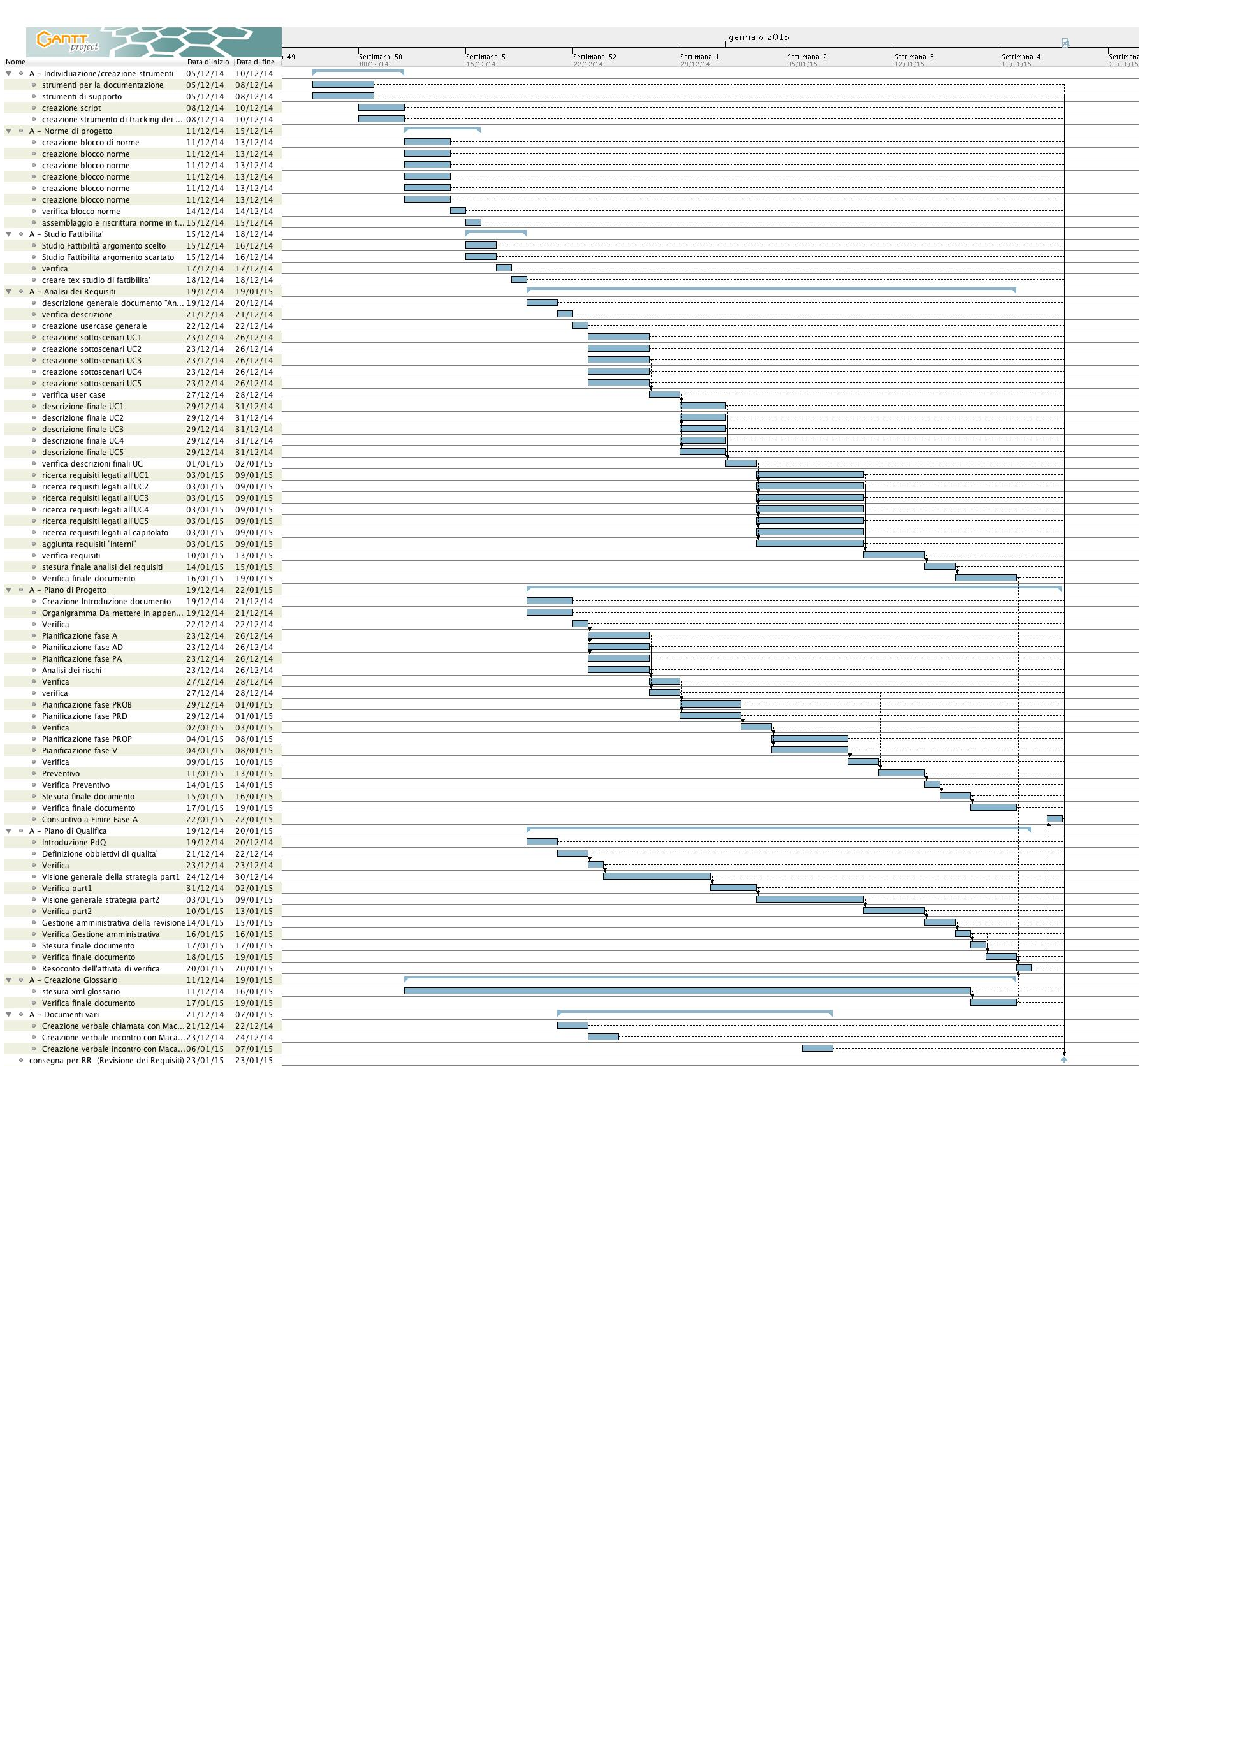
\includegraphics{PianoDiProgetto/Pics/FaseA.pdf}

	% !TEX encoding = UTF-8 Unicode
\subsection{Fase AD: Analisi al Dettaglio}
\textbf{Periodo: dal 16/02/2015 al 22/02/2015}
\\
Questa fase comincia al termine della Fase A di Analisi dei Requisiti. È caratterizzata da una nuova analisi di tutti i documenti redatti nella fase precedente e dalla correzione di questi in base alle richieste e segnalazioni del proponente. Gli analisti provvedono all'individuazione dei nuovi requisiti, la correzione dei requisiti segnalati e si provvede all'incremento di tutti gli altri documenti.
\subsubsection{Diagramma di Gantt delle attività}
\begin{center}
	\begin{figure}[here]\centering
		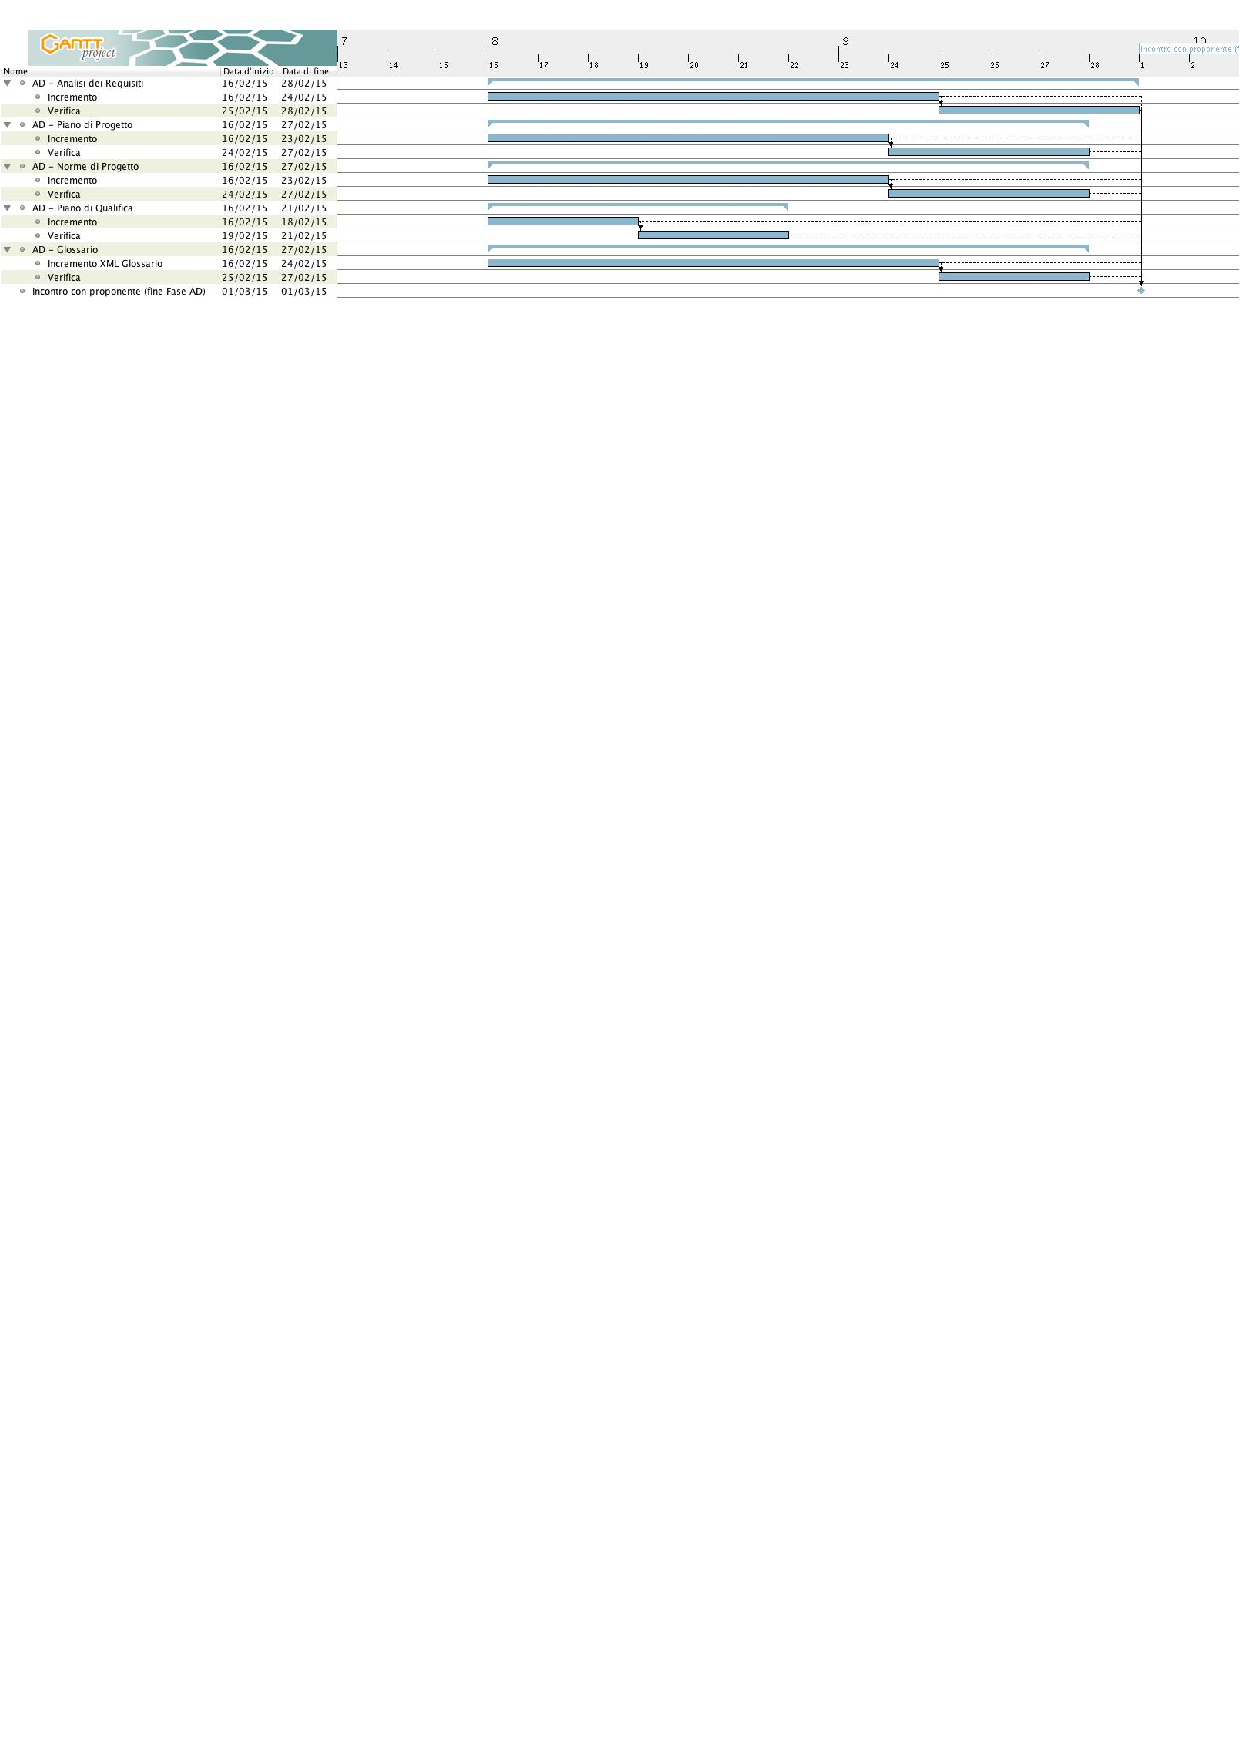
\includegraphics[width=\textwidth]{PianoDiProgetto/Pics/FaseAD}
		\caption{Gantt Fase AD}
	\end{figure}
\end{center}
	% !TEX encoding = UTF-8 Unicode
\subsection{Fase PA}
	\textbf{Periodo}: dal \insdate{23}{02}{2015} al \insdate{16}{03}{2015} \\Questa fase comincia con la fine della \insphase{Fase AD} e termina con l'incontro con il proponente per mostrare l'architettura scelta. \\Le attività di questa fase sono:
	\begin{itemize}
		\item \textbf{Norme Di Progetto}: Viene fatto un incremento alle norme per poter stendere il documento \insdoc{Specifica Tecnica v1.0}. Viene successivamente fatta una verifica/validazione per fissare una baseline al documento che diventerà \insfile{Norme Di Progetto v2.0}.
		\item \textbf{Specifica Tecnica}: Questa attività caratterizza la \insphase{Progettazione Architetturale}. Il \insrole{Progettista} stende la \insdoc{Specifica Tecnica} che contiene le scelte progettuali, ad alto livello, che il progetto dovrà avere. Saranno quindi descritti quali design pattern \projectname{} implementerà, l'architettura generale del software, i principali flussi di controllo e il tracciamento dei requisiti.
		\item \textbf{Glossario}: Viene fatto un incremento al Glossario aggiungendo tutti i vocaboli che si ritiene importante siano inclusi. Viene successivamente fatta una verifica/validazione per fissare una baseline al documento che diventerà \insfile{Glossario v3.0}.
		\item \textbf{Piano Di Qualifica}: L'incremento consiste nell'aggiungere al documento \insfile{Piano Di Qualifica v1.0} il dettaglio dell'esito della \insrev{Revisione dei Requisiti} e la parte della pianificazione dei test. Questa attività genererà, dopo una verifica e validazione, il file \insfile{Piano Di Qualifica v2.0}.
		\item \textbf{Piano di Progetto}: l'incremento che sarà fatto al documento \insdoc{Piano Di Progetto} in questa fase consiste nell'apportare correzioni nella divisione delle attività e stillare il consuntivo di questo periodo. Dopo un'accurata verifica che fisserà una nuova baseline e la validazione il documento diventerà \insfile{Piano Di Progetto v2.0}.
	\end{itemize}
	\subsubsection{Diagramma di Gantt delle attività}
	\begin{figure}\centering
		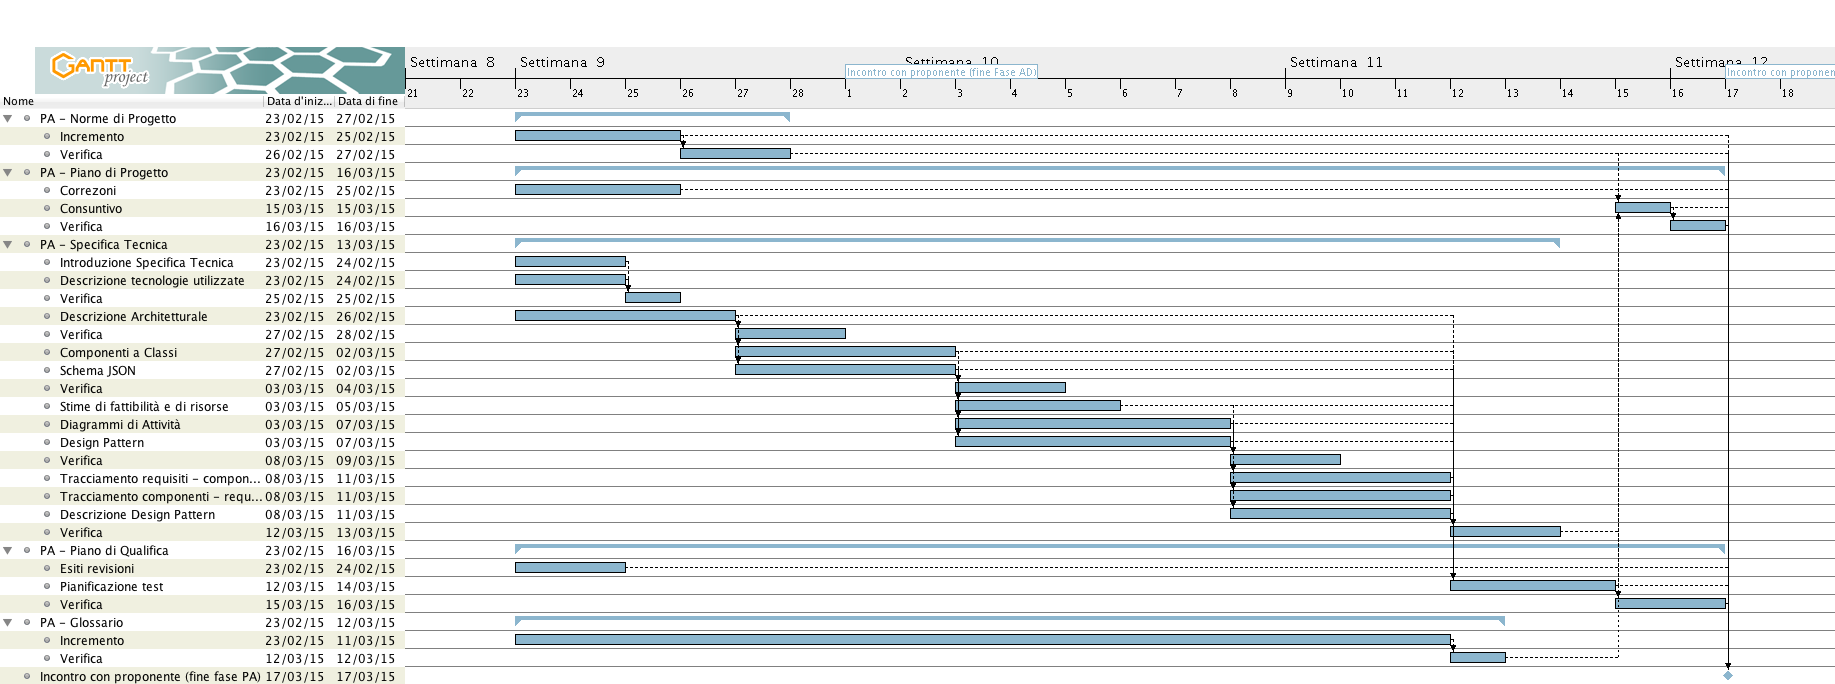
\includegraphics[scale=0.27]{PianoDiProgetto/Pics/FasePA.png}
	\caption{titolo}
\end{figure}
	% !TEX encoding = UTF-8 Unicode
\subsection{Fase PROB: Progettazione Requisiti OBbligatori}
	\textbf{Periodo}: dal \insdate{16}{03}{2015} al \insdate{08}{04}{2015} \\Questa fase comincia con la fine della \insphase{Fase PA} e termina con l'incontro con il proponente al fine di mostrare il prototipo con i requisiti obbligatori sviluppati.\\Le attività di questa fase saranno le seguenti:
	\begin{itemize}
		\item\textbf{Definizione Di Prodotto}: Viene steso il documento \insfile{Definizione di Prodotto v1.0}. Esso definisce la struttura interna del sistema e le relazioni dei componenti del prodotto relativi ai requisiti obbligatori.
		\item\textbf{Manuale Utente e Manuale Amministratore}: Comincia la stesura dei manuali che forniranno indicazioni agli utilizzatori del sistema.
		\item\textbf{Incremento e Verifica Documenti}: Vengono eseguite modifiche ai documenti già scritti, se necessario.
		\item\textbf{Glossario}: Vengono aggiunti al file \insfile{Glossario.xml} i vocaboli dei quali si ritiene necessaria una definizione formale. Alla fine di questa fase vieni quindi generato il documento \insdoc{Glossario v4.0}.
	\end{itemize}
	\subsubsection{Diagramma di Gantt delle attività}
	\begin{figure}[H]\centering
		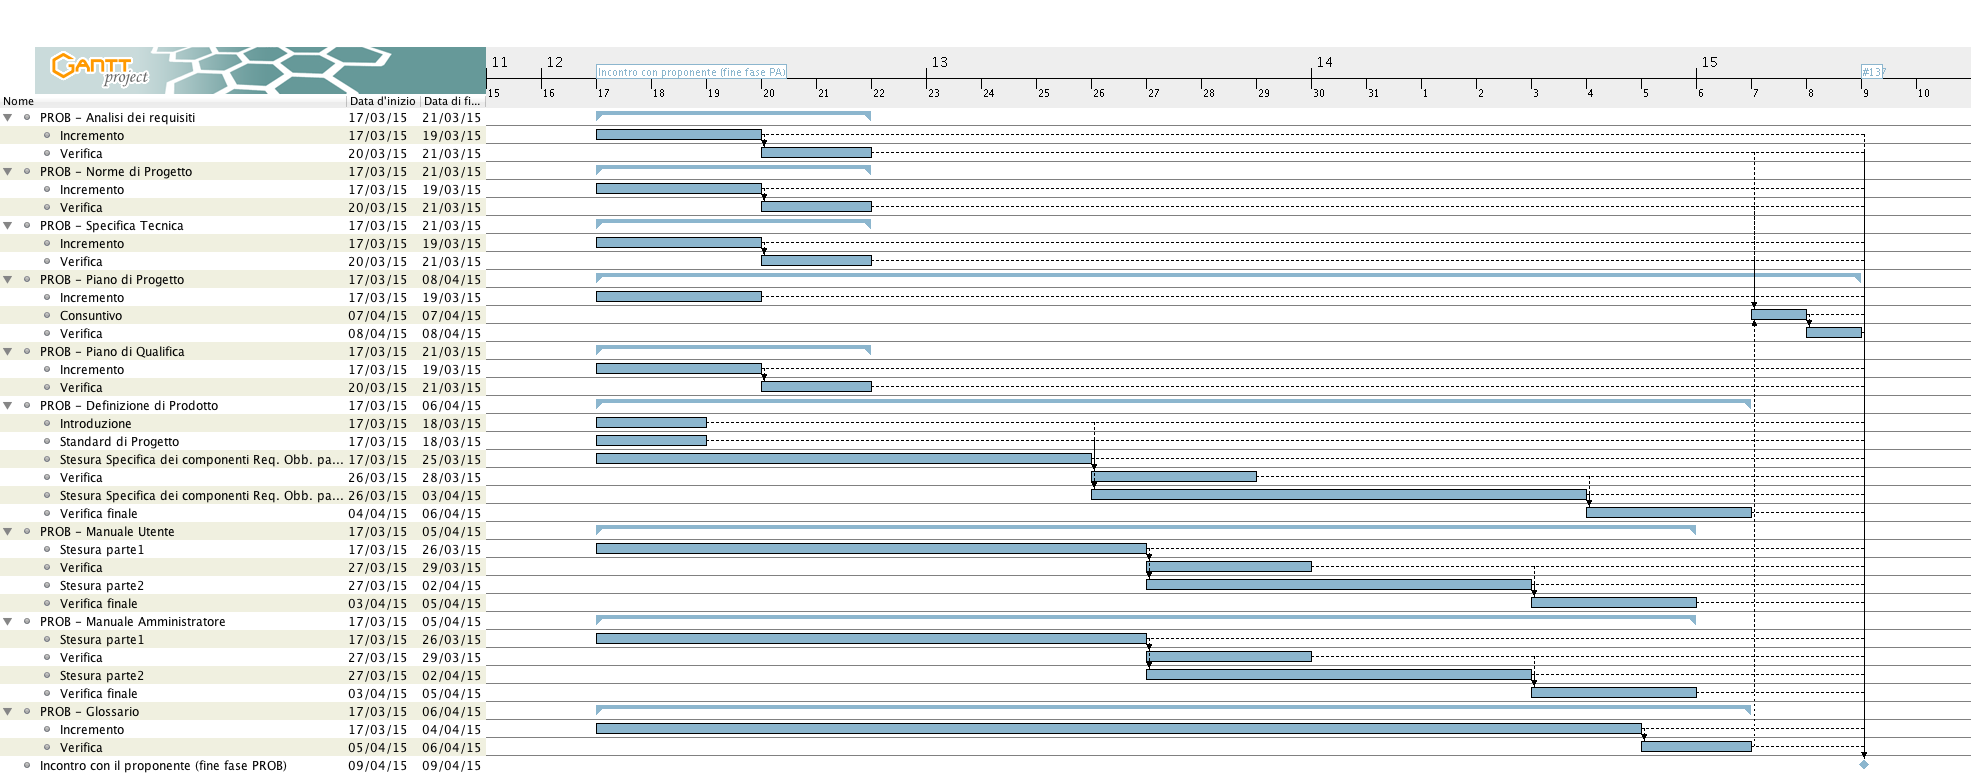
\includegraphics[width=\textwidth]{PianoDiProgetto/Pics/FasePROB.png}
	\caption{Gantt Fase PROB}
\end{figure}
	\subsection{Fase PRD}
	\textbf{Periodo}: dal \insdate{08}{04}{2015} al \insdate{19}{04}{2015} \\Questa fase comincia con la fine della \insphase{Fase PROB} e termina con la scadenza della consegna della \insrev{Revisione Di Progetto}.\\Le attività di questa fase saranno le seguenti:
	\begin{itemize}
		\item\textbf{Definizione di Prodotto}: Viene steso il documento \insfile{Definizione Di Prodotto v2.0}. Esso definisce la struttura interna del sistema e le relazioni dei componenti del prodotto relativi ai requisiti desiderabili.
		\item\textbf{Manuale Utente e Manuale Amministratore}: Comincia la stesura dei manuali che forniranno indicazioni agli utilizzatori del sistema.
		\item\textbf{Incremento e Verifica Documenti}: Vengono eseguite modifiche ai documenti già scritti, se necessario.
		\item\textbf{Glossario}: Vengono aggiunti al file \insfile{Glossario.xml} i vocaboli dei quali si ritiene necessaria una definizione formale. Alla fine di questa fase vieni quindi generato il documento \insdoc{Glossario v5.0}.
	\end{itemize}
	\subsubsection{Diagramma di Gantt delle attività}
	\begin{figure}\centering
		%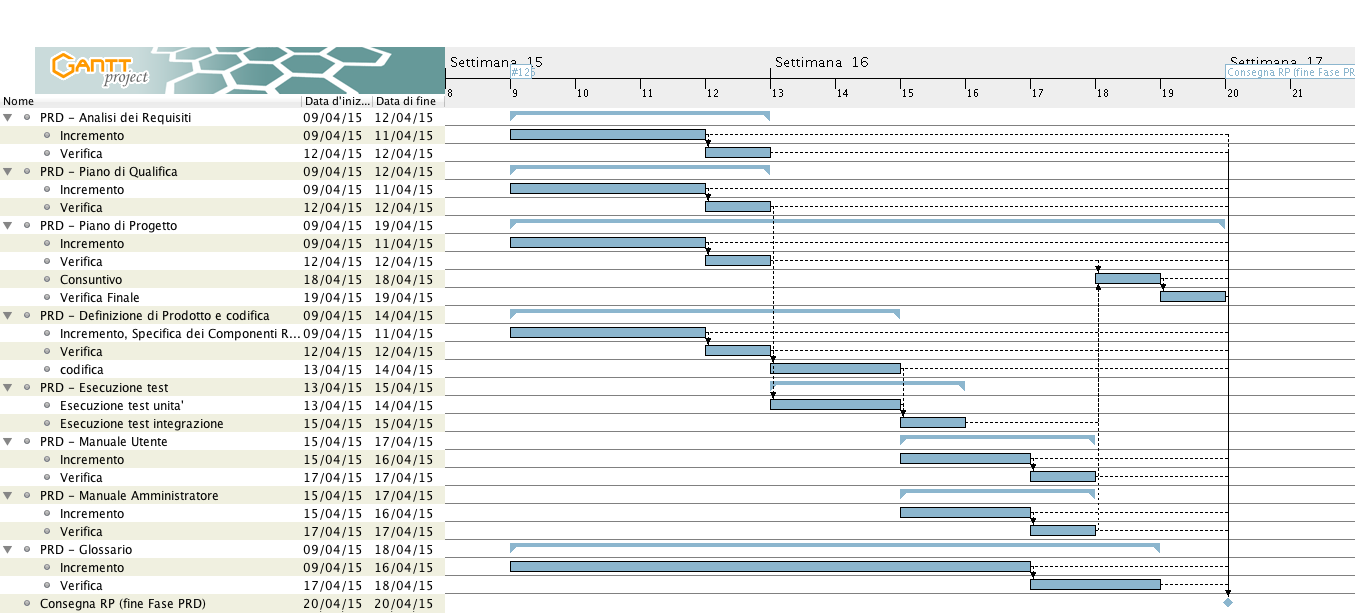
\includegraphics{PianoDiProgetto/Pics/FasePRD.png}
	\caption{titolo}
\end{figure}
	\subsection{Fase PROP: Progettazione Requisiti OPzionali}
	\textbf{Periodo}: dal \insdate{19}{04}{2015} al \insdate{07}{05}{2015} \\Questa fase comincia subito dopo la scadenza della consegna per la \insrev{Revisione Di Progetto} e termina con l'incontro con il proponente al fine di mostrare il prototipo con tutti i requisiti (obbligatori, desiderabili e opzionali) sviluppati. 
	\\Le attività di questa fase saranno le seguenti:
	\begin{itemize}
		\item\textbf{Definizione Di Prodotto}: Viene steso il documento \insfile{Definizione di Prodotto v3.0}. Esso definisce la struttura interna del sistema e le relazioni dei componenti del prodotto relativi ai requisiti opzionali.
		\item\textbf{Manuale Utente e Manuale Amministratore}: Comincia la stesura dei manuali che forniranno indicazioni agli utilizzatori del sistema.
		\item\textbf{Incremento e Verifica Documenti}: Vengono eseguite modifiche ai documenti già scritti, se necessario.
		\item\textbf{Glossario}: Vengono aggiunti al file \insfile{Glossario.xml} i vocaboli dei quali si ritiene necessaria una definizione formale. Alla fine di questa fase vieni quindi generato il documento \insdoc{Glossario v6.0}.
	\end{itemize}
	\subsubsection{Diagramma di Gantt delle attività}
	\begin{figure}\centering
		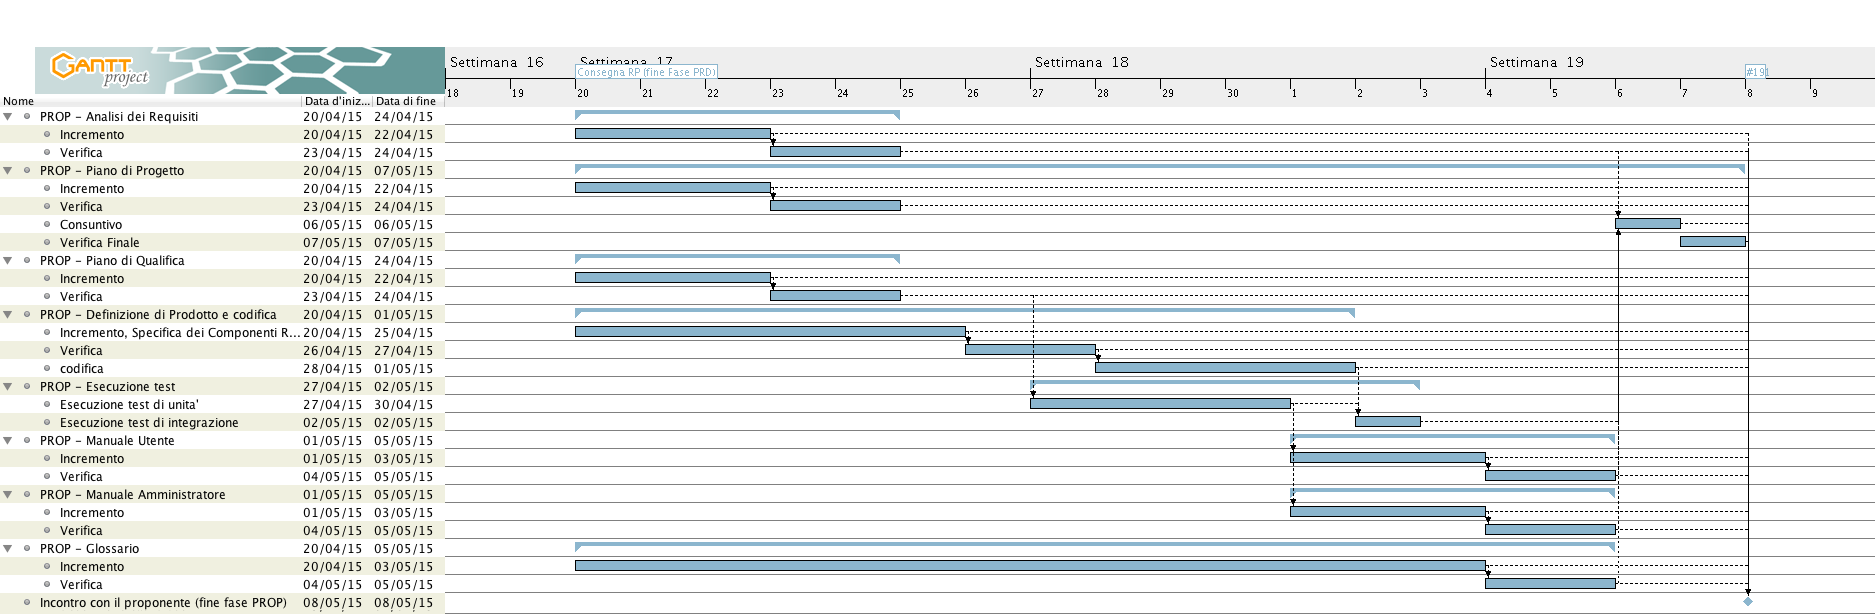
\includegraphics[width=\textwidth]{PianoDiProgetto/Pics/FasePROP.png}
	\caption{Gantt Fase PROP}
\end{figure}
	% !TEX encoding = UTF-8 Unicode
\subsection{Fase V: Validazione}
	\textbf{Periodo}: dal \insdate{10}{05}{2015} al \insdate{07}{06}{2015} \\Questa fase comincia con la fine della \insphase{Fase PROP} e termina con la scadenza della consegna per la \insrev{RA}.
	\begin{itemize}
		\item \textbf{Incremento e Verifica}: se necessario verranno effettuati aggiornamenti ai vari documenti scritti;
		\item \textbf{Validazione}: viene verificato, attraverso tracciamento, di aver soddisfatto i requisiti presenti nel documento \insdoc{Analisi dei Requisiti v1.00};
		\item \textbf{Esecuzione test}: verranno eseguiti i test di sistema previsti dal documento \insdoc{Piano di Qualifica v 7.00};
		\item \textbf{Correzione bug}: i bug rilevati verranno risolti;
		\item \textbf{Collaudo}: viene eseguito e completamente collaudato il sistema creato.
	\end{itemize}
	\subsubsection{Diagramma di Gantt delle attività}
		\begin{figure}[H]\centering
			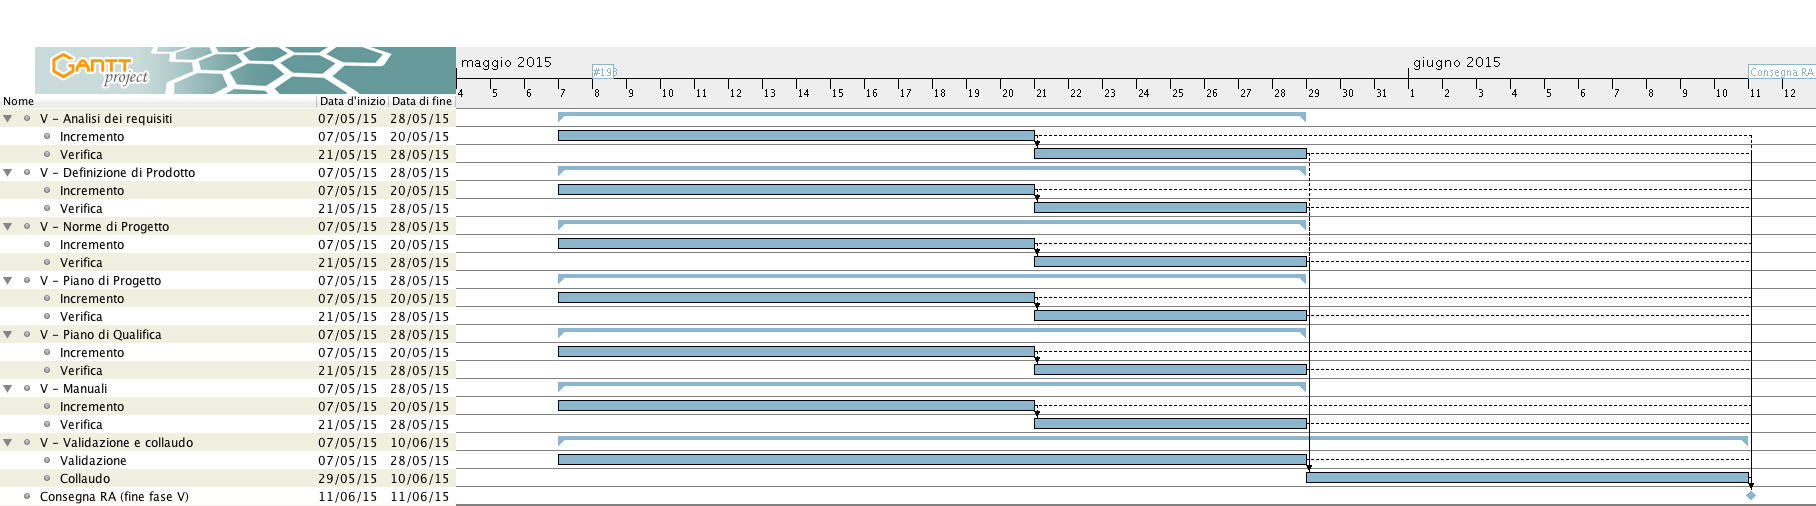
\includegraphics[width=\textwidth]{PianoDiProgetto/Pics/FaseV.png}
		\caption{Gantt Fase V}
\end{figure}

	
